%\documentclass[hyperref={pdfpagelabels=false},slidetop,9pt]{beamer}
\documentclass[slidetop,8pt]{beamer}
\usepackage[T1]{fontenc}
\usepackage[utf8]{inputenc}
\newcommand{\id}{54}
\newcommand{\nom}{Liaisons mécaniques}
\newcommand{\sequence}{04}
\newcommand{\num}{01}
\newcommand{\type}{TP}
\newcommand{\descrip}{Modélisation d'un solide. Comportement des liaisons mécaniques. Modéliser les mécanismes du laboratoire par un schéma cinématique, paramétré.}
\newcommand{\competences}{A3-C4: Analyse d'architecture et de comportement \\ &  Mod1-C1: Isolement d'un solide ou d'un système de solides \\ &  Mod2-C10-1: Modèle de solide indéformable \\ &  Mod2-C11: Modélisation géométrique et cinématique des mouvements entre solides indéformables \\ &  Mod2-C12: Modélisation cinématique des liaisons entre solides \\ &  Mod2-C15: Modélisation des actions mécaniques \\ &  Rés-C6: Utilisation d'un solveur ou d'un logiciel multi physique \\ &  Com1-C1: Différents descripteurs introduits dans le programme \\ &  Com2-C4: Outils de communication}
\newcommand{\nbcomp}{9}
\newcommand{\systemes}{Plateforme Stewart}
\newcommand{\systemessansaccent}{Plateforme Stewart}
\newcommand{\ilot}{2}
\newcommand{\ilotstr}{02}
\newcommand{\dossierilot}{\detokenize{Ilot_02 Plateforme Stewart}}
\newcommand{\imageun}{Plateforme}

\newcommand{\urlsysteme}{\href{https://www.costadoat.fr/systeme/57}{Ressources système}}
\newcommand{\matlabsimscape}{\href{https://github.com/Costadoat/Sciences-Ingenieur/raw/master/Systemes/Plateforme Stewart/Plateforme_Stewart_Simscape.zip}{Modèle Simscape}}
\newcommand{\solidworks}{\href{https://github.com/Costadoat/Sciences-Ingenieur/raw/master/Systemes/Plateforme Stewart/Plateforme_Stewart_Solidworks.zip}{Modèle Solidworks}}
\newcommand{\edrawings}{\href{https://github.com/Costadoat/Sciences-Ingenieur/raw/master/Systemes/Plateforme Stewart/Plateforme_Stewart.EASM}{Modèle eDrawings}}
\newcommand{\test}{Stewart_param1}
\newcommand{\testi}{Stewart_param2}
\newcommand{\testii}{Stewart_param3}
\newcommand{\testiii}{Stewart_param4}
\newcommand{\testiiii}{Stewart_euler}
\usepackage{etex}
\usepackage{tikz}
\usepackage[european]{circuitikz}
\usepackage{pgf}
\usepackage[all]{xy}
\usepackage{pgfpages}
\usepackage{graphbox}
\usepackage{pdfpages}
\usepackage[adobe-utopia]{mathdesign}
\usepackage{ifthen}
\usepackage{cancel}
\usepackage{framed}
\usepackage{subfig}
\usepackage{tabularx}
\usepackage{setspace}
\usepackage{soul}
\usepackage{schemabloc}
\usepackage{eqnarray}
\usepackage[dot, phantomtext]{dashundergaps}
\usepackage{media9}
\usepackage{multimedia}
\usepackage{textcomp}

\author{Renaud Costadoat}
\institute{Lycée Dorian}

\usepackage{multido}
\usepackage{multirow}
\usepackage{multicol} % Portions de texte en colonnes
\usepackage{flafter}%floatants après la référence

\usepackage{color}
\usepackage{xcolor}
\usepackage{colortbl}

\usepackage[gen]{eurosym}
\usepackage{tikz}
%\usepackage{pstricks,pst-node,pst-tree,pst-solides3d}
\usepackage{lmodern}
\usepackage[francais]{babel}
\usepackage{pslatex}
\usetheme{renaud}
\usepackage{times}
\usepackage{amsmath}
\usepackage{verbatim}
\usepackage{moreverb}
%\usetikzlibrary{arrows,shapes}
\usepackage{graphicx}
\usepackage{psfrag}
\usepackage{wrapfig}
\usepackage{etoolbox}

\definecolor{gris25}{gray}{0.75}
\definecolor{bleu}{RGB}{18,33,98}
\definecolor{bleuf}{RGB}{42,94,171}
\definecolor{bleuc}{RGB}{231,239,247}
\definecolor{rougef}{RGB}{185,18,27}
\definecolor{rougec}{RGB}{255,188,204}%255,230,231
\definecolor{vertf}{RGB}{103,126,82}
\definecolor{vertc}{RGB}{220,255,191}

\setlength\parindent{24pt}
\parskip 7.2pt
\parindent 8pt

\newenvironment{rem}[1][\hsize]%
{%
    \def\FrameCommand
   {%
\rotatebox{90}{\textit{\textsf{Remarque}}} 
       {\color{bleuf}\vrule width 3pt}%
       \hspace{0pt}%must no space.
       \fboxsep=\FrameSep\colorbox{bleuc}%
  }%
    \MakeFramed{\hsize#1\advance\hsize-\width\FrameRestore}%
}%
{\endMakeFramed}%


\newenvironment{savoir}[1][\hsize]%
{%
    \def\FrameCommand
    {%
\rotatebox{90}{\textit{\textsf{Savoir}}} 
        {\color{bleuf}\vrule width 3pt}%
        \hspace{0pt}%must no space.
        \fboxsep=\FrameSep\colorbox{bleuc}%
    }%
    \MakeFramed{\hsize#1\advance\hsize-\width\FrameRestore}%
}%
{\endMakeFramed}%

\newenvironment{prob}[1][\hsize]%
{%
    \def\FrameCommand%
    {%
\rotatebox{90}{\textit{\textsf{Problematique}}} 
        {\color{rougef}\vrule width 3pt}%
        \hspace{0pt}%must no space.
        \fboxsep=\FrameSep\colorbox{rougec}%
    }%
    \MakeFramed{\hsize#1\advance\hsize-\width\FrameRestore}%
}%
{\endMakeFramed}%

\newenvironment{obj}[1][\hsize]%
{%
    \def\FrameCommand%
    {%
\rotatebox{90}{\textit{\textsf{Objectif}}} 
        {\color{vertf}\vrule width 3pt}%
        \hspace{0pt}%must no space.
        \fboxsep=\FrameSep\colorbox{vertc}%
    }%
    \MakeFramed{\hsize#1\advance\hsize-\width\FrameRestore}%
}%
{\endMakeFramed}%

\newenvironment{defi}[1][\hsize]%
{%
    \def\FrameCommand%
    {%
\rotatebox{90}{\textit{\textsf{Definition}}} 
        {\color{bleuf}\vrule width 3pt}%
        \hspace{0pt}%must no space.
        \fboxsep=\FrameSep\colorbox{rougec}%
    }%
    \MakeFramed{\hsize#1\advance\hsize-\width\FrameRestore}%
}%
{\endMakeFramed}%


\newenvironment{hypo}[1][\hsize]%
{%
    \def\FrameCommand%
    {%
\rotatebox{90}{\textit{\textsf{Hypothèse\\}}} 
        {\color{bleuf}\vrule width 3pt}%
        \hspace{0pt}%must no space.
        \fboxsep=\FrameSep\colorbox{bleuc}%
    }%
    \MakeFramed{\hsize#1\advance\hsize-\width\FrameRestore}%
}%
{\endMakeFramed}%


\newenvironment{prop}[1][\hsize]%
{%
    \def\FrameCommand%
    {%
\rotatebox{90}{\textit{\textsf{Propriété}}} 
        {\color{bleuf}\vrule width 3pt}%
        \hspace{0pt}%must no space.
        \fboxsep=\FrameSep\colorbox{bleuc}%
    }%
    \MakeFramed{\hsize#1\advance\hsize-\width\FrameRestore}%
}%
{\endMakeFramed}%

\newenvironment{props}[1][\hsize]%
{%
    \def\FrameCommand%
    {%
\rotatebox{90}{\textit{\textsf{Propriétés}}} 
        {\color{bleuf}\vrule width 3pt}%
        \hspace{0pt}%must no space.
        \fboxsep=\FrameSep\colorbox{bleuc}%
    }%
    \MakeFramed{\hsize#1\advance\hsize-\width\FrameRestore}%
}%
{\endMakeFramed}%

\newenvironment{exemple}[1][\hsize]%
{%
    \def\FrameCommand%
    {%
\rotatebox{90}{\textit{\textsf{Exemple}}} 
        {\color{vertf}\vrule width 3pt}%
        \hspace{0pt}%must no space.
        \fboxsep=\FrameSep\colorbox{vertc}%
    }%
    \MakeFramed{\hsize#1\advance\hsize-\width\FrameRestore}%
}%
{\endMakeFramed}%

\newenvironment{resultat}[1][\hsize]%
{%
    \def\FrameCommand%
    {%
\rotatebox{90}{\textit{\textsf{Résultat}}} 
        {\color{rougef}\vrule width 3pt}%
%        {\color{bleuf}\vrule width 3pt}%
        \hspace{0pt}%must no space.
        \fboxsep=\FrameSep\colorbox{rougec}%
    }%
    \MakeFramed{\hsize#1\advance\hsize-\width\FrameRestore}%
}%
{\endMakeFramed}%

\newenvironment{methode}[1][\hsize]%
{%
    \def\FrameCommand%
    {%
\rotatebox{90}{\textit{\textsf{Méthode\\}}} 
        {\color{rougef}\vrule width 3pt}%
        \hspace{0pt}%must no space.
        \fboxsep=\FrameSep\colorbox{rougec}%
    }%
    \MakeFramed{\hsize#1\advance\hsize-\width\FrameRestore}%
}%
{\endMakeFramed}%

\newenvironment{theo}[1][\hsize]%
{%
    \def\FrameCommand%
    {%
\rotatebox{90}{\textit{\textsf{Théorème\\}}} 
        {\color{rougef}\vrule width 3pt}%
        \hspace{0pt}%must no space.
        \fboxsep=\FrameSep\colorbox{rougec}%
    }%
    \MakeFramed{\hsize#1\advance\hsize-\width\FrameRestore}%
}%
{\endMakeFramed}%

\newenvironment{warn}[1][\hsize]%
{%
    \def\FrameCommand%
    {%
\rotatebox{90}{\textit{\textsf{Attention\\}}} 
        {\color{rougef}\vrule width 3pt}%
        \hspace{0pt}%must no space.
        \fboxsep=\FrameSep\colorbox{rougec}%
    }%
    \MakeFramed{\hsize#1\advance\hsize-\width\FrameRestore}%
}%
{\endMakeFramed}%

% \usepackage{pstricks}
%\usepackage{minitoc}
% \setcounter{minitocdepth}{4}

\setcounter{tocdepth}{2}

% \mtcselectlanguage{french} 

%\usepackage{draftcopy}% "Brouillon"
% \usepackage{floatflt}
\usepackage{psfrag}
%\usepackage{listings} % Permet d'insérer du code de programmation
\renewcommand{\baselinestretch}{1.2}

% Changer la num�rotation des figures :
% ------------------------------------
% \makeatletter
% \renewcommand{\thefigure}{\ifnum \c@section>\z@ \thesection.\fi
%  \@arabic\c@figure}
% \@addtoreset{figure}{section}
% \makeatother
 


%%%%%%%%%%%%
% Définition des vecteurs %
%%%%%%%%%%%%
 \newcommand{\vect}[1]{\overrightarrow{#1}}

%%%%%%%%%%%%
% Définition des torseusr %
%%%%%%%%%%%%

 \newcommand{\torseur}[1]{%
\left\{{#1}\right\}
}

\newcommand{\torseurcin}[3]{%
\left\{\mathcal{#1} \left(#2/#3 \right) \right\}
}

\newcommand{\torseurstat}[3]{%
\left\{\mathcal{#1} \left(#2\rightarrow #3 \right) \right\}
}

 \newcommand{\torseurc}[8]{%
%\left\{#1 \right\}=
\left\{
{#1}
\right\}
 = 
\left\{%
\begin{array}{cc}%
{#2} & {#5}\\%
{#3} & {#6}\\%
{#4} & {#7}\\%
\end{array}%
\right\}_{#8}%
}

 \newcommand{\torseurcol}[7]{
\left\{%
\begin{array}{cc}%
{#1} & {#4}\\%
{#2} & {#5}\\%
{#3} & {#6}\\%
\end{array}%
\right\}_{#7}%
}

 \newcommand{\torseurl}[3]{%
%\left\{\mathcal{#1}\right\}_{#2}=%
\left\{%
\begin{array}{l}%
{#1} \\%
{#2} %
\end{array}%
\right\}_{#3}%
}

 \newcommand{\vectv}[3]{%
\vect{V\left( {#1} \in {#2}/{#3}\right)}
}


\newcommand{\vectf}[2]{%
\vect{R\left( {#1} \rightarrow {#2}\right)}
}

\newcommand{\vectm}[3]{%
\vect{\mathcal{M}\left( {#1}, {#2} \rightarrow {#3}\right)}
}


 \newcommand{\vectg}[3]{%
\vect{\Gamma \left( {#1} \in {#2}/{#3}\right)}
}

 \newcommand{\vecto}[2]{%
\vect{\Omega\left( {#1}/{#2}\right)}
}

\newcommand{\reponse}[1][4]
{
\multido{}{#1}
{
\begin{center}
\makebox[0.9\linewidth]{\dotfill} \end{center}
}}


% }$$\left\{\mathcal{#1} \right\}_{#2} =%
% \left\{%
% \begin{array}{c}%
%  #3 \\%
%  #4 %
% \end{array}%
% \right\}_{#5}}


%  ------------------------------------------
% | Modification du formatage des sections : | 
%  ------------------------------------------

% Grands titres :
% ---------------

\newcommand{\titre}[1]{%
\begin{center}
      \bigskip
      \rule{\textwidth}{1pt}
      \par\vspace{0.1cm}
      
      \textbf{\large #1}
      \par\rule{\textwidth}{1pt}
    \end{center}
    \bigskip
  }

% Supprime le numéro du chapitre dans la numérotation des sections:
% -----------------------------------------------------------------
\makeatletter
\renewcommand{\thesection}{\@arabic\c@section}
\makeatother


% \titleformat{\chapter}[display]
% {\normalfont\Large\filcenter}
% {}
% {1pc}
% {\titlerule[1pt]
%   \vspace{1pc}%
%   \Huge}[\vspace{1ex}%
% \titlerule]


%%%% Chapitres Comme PY Pechard %%%%%%%%%
% numéro du chapitre
\DeclareFixedFont{\chapnumfont}{OT1}{phv}{b}{n}{80pt}
% pour le mot " Chapitre "
\DeclareFixedFont{\chapchapfont}{OT1}{phv}{m}{it}{40pt}
% pour le titre
\DeclareFixedFont{\chaptitfont}{T1}{phv}{b}{n}{25pt}

\definecolor{gris}{gray}{0.75}
\setbeamertemplate{section in toc}[sections numbered]

\newlength{\RoundedBoxWidth}
\newsavebox{\GrayRoundedBox}
\newenvironment{GrayBox}[1][\dimexpr\textwidth-4.5ex]%
   {\setlength{\RoundedBoxWidth}{\dimexpr#1}
    \begin{lrbox}{\GrayRoundedBox}
       \begin{minipage}{\RoundedBoxWidth}}%
   {   \end{minipage}
    \end{lrbox}
    \begin{center}
    \begin{tikzpicture}%
       \draw node[draw=bleuf,fill=bleuc,rounded corners,%
             inner sep=2ex,text width=\RoundedBoxWidth]%
             {\usebox{\GrayRoundedBox}};
    \end{tikzpicture}
    \end{center}}
    
\ifdef{\prive}{\pgfpagesuselayout{2 on 1}[a4paper,border shrink=0mm]}
\ifdef{\prive}{\setbeamertemplate{navigation symbols}{}}
\setbeamertemplate{itemize item}[ball]
%\setbeamertemplate{blocks}[rounded]%[shadow=true]
\setbeamercolor{block title}{fg=white,bg=grisf}        % titre block normal 
\setbeamercolor{block body}{fg=grisf,bg=grisc!50}      % corps block normal
\setbeamercolor{block body alerted}{fg=white,bg=warning}   % idem pour un block alerte

\title{\nom}
\date{S\sequence \ - \type\num}

\begin{document}
\shorthandoff{:!}
\bibliographystyle{abbrvnat-fr}

\usebackgroundtemplate%
{%
    \centering
\includegraphics[width=\paperwidth]{../../img/fond2}%
}

{
\setbeamertemplate{navigation symbols}{}
\setbeamertemplate{headline}[pagetitre]
\setbeamertemplate{footline}[pagetitre]
\usebackgroundtemplate{\centering
\includegraphics[width=\paperwidth]{../../img/fond}}
\frame{\titlepage}
}



\setcounter{framenumber}{0}

{\frame{
\frametitle{Introduction}

\begin{savoir}
Vous êtes capables :
\begin{itemize}
 \item De définir et de lire des spécifications sur un dessin de définition.
\end{itemize}
\end{savoir}

\begin{prob}
Vous devez êtes capables :
\begin{itemize}
 \item De contrôler ces spécifications sur une pièce fabriquée.
\end{itemize}
\end{prob}
}}

\section{Introduction}

{\frame{
\frametitle{Inspection d'une spécification portée sur un dessin}

\begin{minipage}{0.65\linewidth}
\begin{itemize}
 \item Les étapes :
\begin{itemize}
 \item Définir selon la norme (ISO) la spécification à contrôler,
 \item Mesurer les surfaces par des points,
 \item Représenter les éléments tolérancés et de références,
 \item Construire les références spécifiées,
 \item Vérifier les spécifications par constructions géométriques et calculs de distances et d'angles,
 \item Estimer les incertitudes sur les caractéristiques.
\end{itemize}
\item Difficultés:
\begin{itemize}
 \item Limites physiques : accessibilité des surfaces.
\end{itemize}
\end{itemize}
\end{minipage}\hfill
\begin{minipage}{0.3\linewidth}
 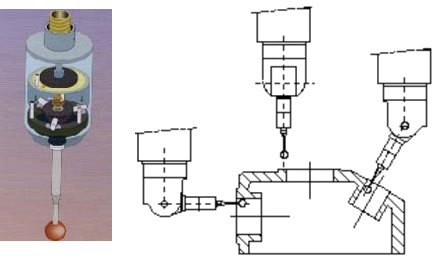
\includegraphics[width=0.9\linewidth]{img/Picture1}
\end{minipage}

 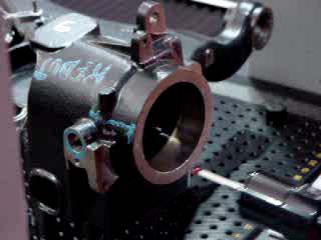
\includegraphics[width=0.25\linewidth]{img/Picture2}\hfill
 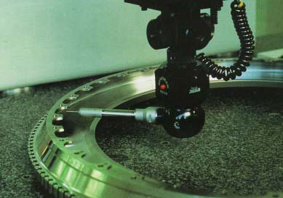
\includegraphics[width=0.25\linewidth]{img/Picture3}\hfill
 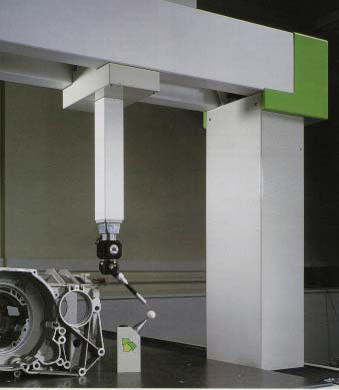
\includegraphics[width=0.25\linewidth]{img/Picture4}
}}

\section{Mesure MMT}

{\frame{
\frametitle{Choisir les outils de mesure sur MMT}

 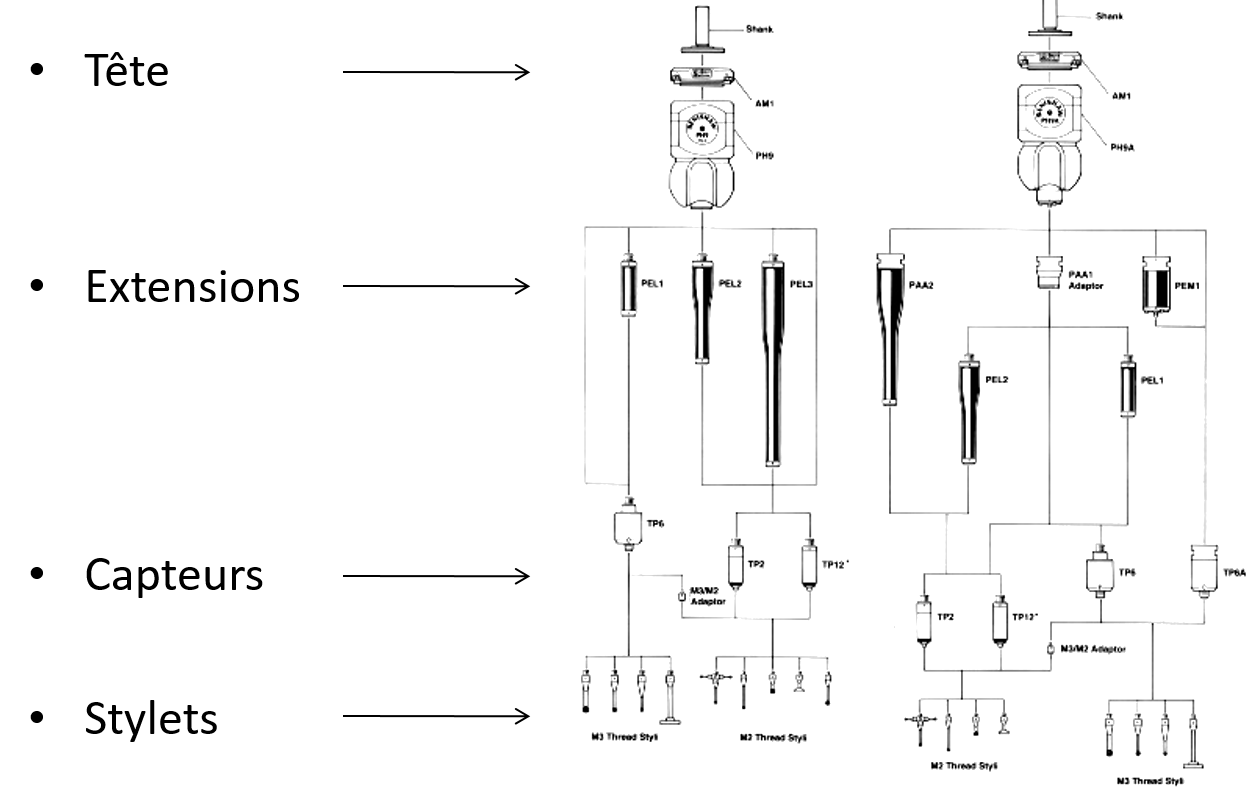
\includegraphics[width=0.9\linewidth]{img/Picture5}
}}

{\frame{
\frametitle{Acquérir des coordonnées de points}

\begin{itemize}
 \item Dans un repère exprimer les coordonnées des points appartenant aux différentes surfaces de la pièce.

\end{itemize}
 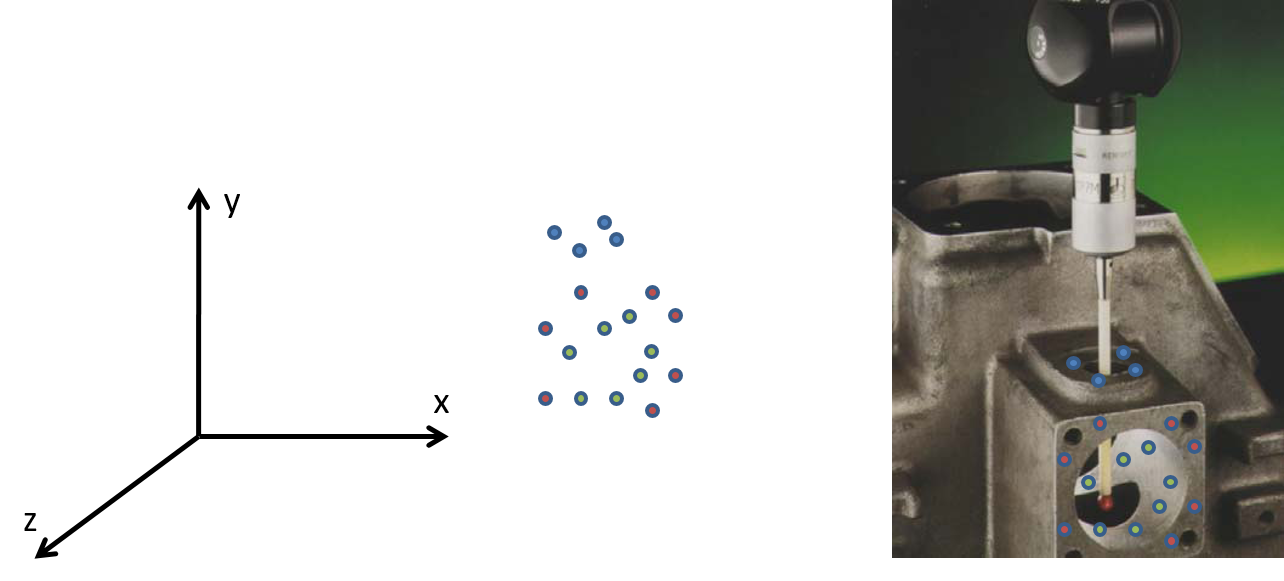
\includegraphics[width=0.9\linewidth]{img/Picture6}
}}

{\frame{
\frametitle{Mesure d'un point}

\begin{itemize}
 \item Les points et les lignes, sont définies par l'intersection d'un élément théorique exact (droite ou plan ) avec la surface portant les points mesurés,
 
 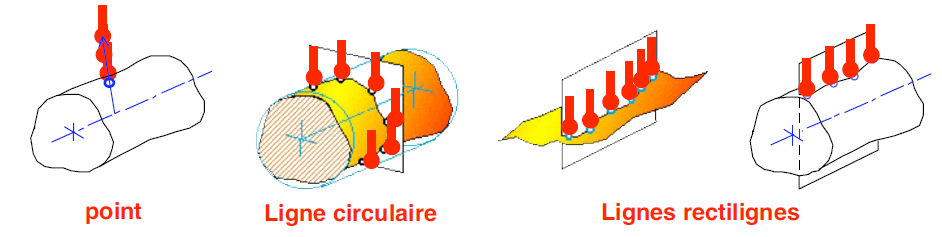
\includegraphics[width=0.9\linewidth]{img/Picture7}
 
 \item Conséquence le déplacement du palpeur doit être contrôlé par la CN de la MMT pour que chaque point de contact avec la surface appartienne au plan de coupe ou à la droite d'intersection,
 \item La mesure des lignes et des points se trouvent ainsi limitées par les possibilités de \og balançage \fg de la pièce dans le repère de la MMT.
\end{itemize}

}}

{\frame{
\frametitle{Qualification d'un palpeur}

\begin{itemize}
 \item Chaque \og outil-palpeur \fg a un rayon qu'il faut compenser par mesure d'un étalon (cale, bague, sphère).
 \begin{itemize}
 \item En mesures unidimensionnelles : par mesure d'une cale étalon de longueur $l_0$,
\begin{center}
 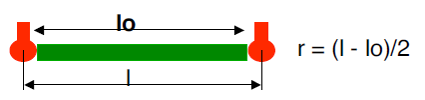
\includegraphics[width=0.4\linewidth]{img/Picture8}
\end{center}
 \item En mesures planes (bidimensionnelles): par mesure d'une bague étalon de diamètre $d_0$,
\begin{center}
 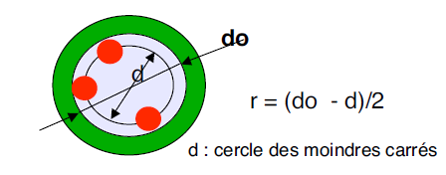
\includegraphics[width=0.4\linewidth]{img/Picture9}
\end{center}
 \item En mesures tridimensionnelles : par mesure d'une sphère étalon de diamètre $d_0$.
\begin{center}
 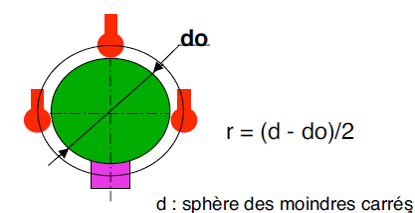
\includegraphics[width=0.4\linewidth]{img/Picture10}
\end{center}
\end{itemize}
\end{itemize}
}}

{\frame{
\frametitle{Représentation d'un élément géométrique réel}

\begin{itemize}
 \item Par l'ensemble des points mesurés sur l'élément (Nuage de points),
\begin{center}
 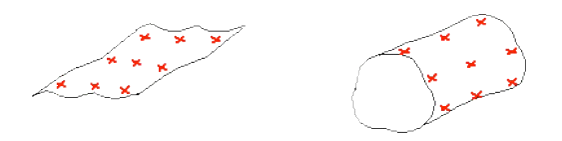
\includegraphics[width=0.6\linewidth]{img/Picture11}
\end{center}
 \item Par un élément géométrique théorique associé au nuage de points suivant le critère des moindres carrés et à la demande (option) tangent du côté libre de la matière.
\begin{center}
 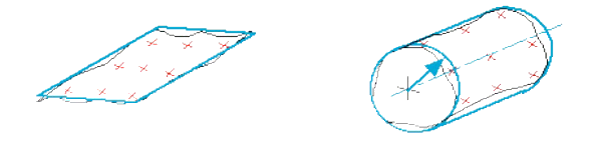
\includegraphics[width=0.6\linewidth]{img/Picture12}
\end{center}
\end{itemize}
}}

{\frame{
\frametitle{Critère des moindres carrés (ou critère de Gauss)}

\begin{itemize}
 \item L'élément associé est tel que la somme des carrés des distances des points mesurés à l'élément est minimale,
\begin{center}
 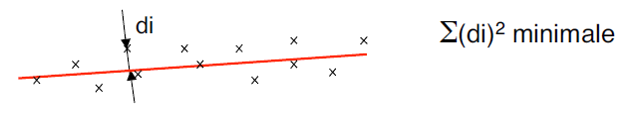
\includegraphics[width=0.6\linewidth]{img/Picture13}
\end{center}
 \item L'élément associé passe au mieux des points. Il est dans le nuage de points. 
L'élément retenu pourra être un élément tangent extérieur matière et parallèle à l'élément des moindres carrés.
\begin{center}
 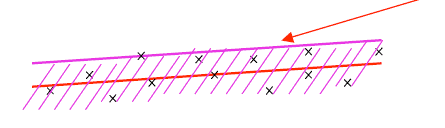
\includegraphics[width=0.6\linewidth]{img/Picture14}
\end{center}
\end{itemize}
}}

{\frame{
\frametitle{Exemple: Couvercle de l'arbre intermédiaire}

\begin{center}
 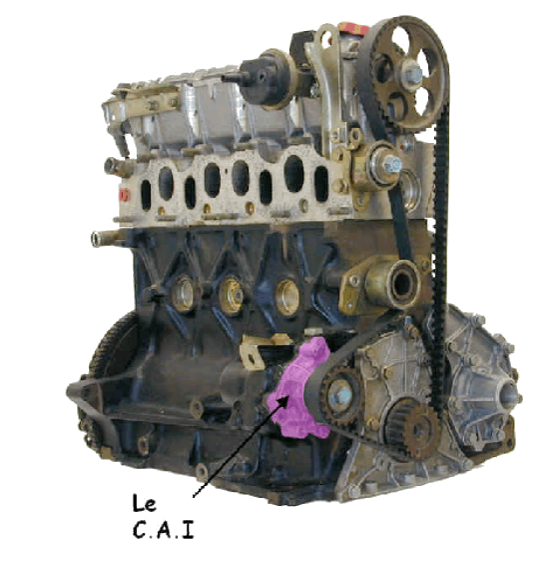
\includegraphics[width=0.65\linewidth]{img/Picture15}
\end{center}
}}

{\frame{
\frametitle{Dessin de définition}

\begin{center}
 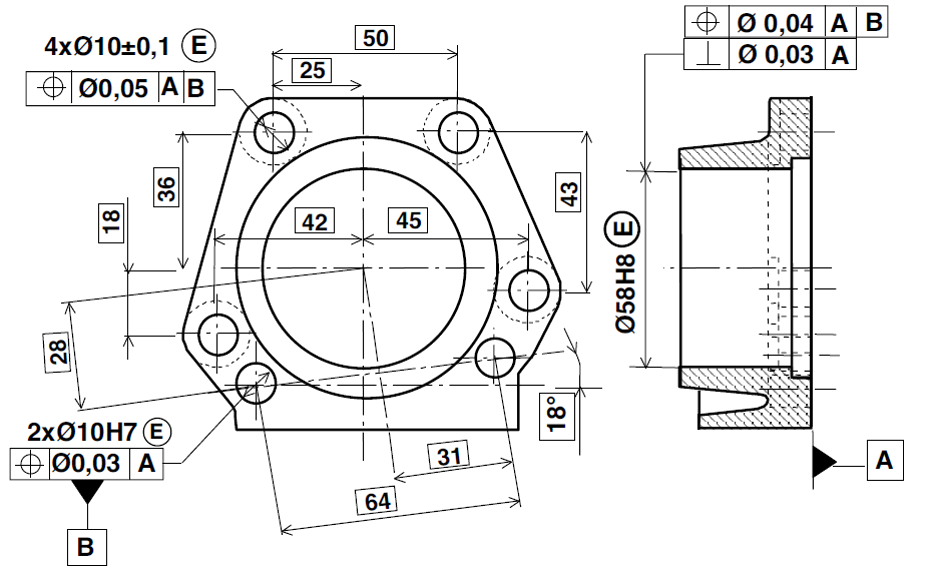
\includegraphics[width=0.9\linewidth]{img/Picture16}
\end{center}
}}

{\frame{
\frametitle{Contrôle d'une spécification dimensionnelle $\Phi 58$}

\begin{itemize}
 \item Définition ISO de la spécification,
 \begin{itemize}
  \item Toutes les dimensions locales réelles doivent être $58,000 \leq di \leq 58,033$,
  \item Exigence de l'enveloppe : la surface réelle doit être extérieure a un cylindre de forme parfaite de diamètre au maximum de matière ($\Phi 58,000$),
 \end{itemize}
 \item Mesure de la surface réputée cylindrique et modèle géométrique associé mesure en 12 points repartis sur la surface,
 \begin{itemize}
  \item modèle associé : cylindre des moindres carres tangent extérieur matière,
  \item résultat : diamètre $D$ du cylindre associé et défaut de forme $df$ sur les 12 pts,
 \end{itemize}
 \item Interprétation du résultat,
 \begin{itemize}
  \item Dimensions locales réelles : vérifier si $D \geq 58,000$ et $(D + 2df) \leq 58,033$,
  \item Exigence de l'enveloppe : vérifier si $D \geq 58,000$,
 \end{itemize}
 \item Incertitude sur la mesure de la caractéristique.
\end{itemize}
}}

{\frame{
\frametitle{Contrôle d'une spécification géométrique 
\includegraphics[height=0.4cm]{img/Picture17}}

\begin{itemize}
 \item Définition ISO de la spécification
 \begin{itemize}
  \item Elément tolérancé : axe reel de l'alesage $\Phi 58$,
  \item Eléments de référence : surface réputée plane A,
  \item Référence spécifiée : plan A tangent extérieur matière et critère des moindres carrés,
  \item Zone de tolérance : Cylindre $\Phi 0,03$ d'axe perpendiculaire au plan de référence spécifié A,
 \end{itemize}
 \item Mesure des surfaces et modèles géométriques de la base de données,
 \begin{itemize}
  \item Mesure en 12 points repartis sur l'alésage,
  \begin{itemize}
   \item Modèle associé : cylindre des moindres carres tangent extérieur matière $CY1$,
  \end{itemize}
  \item Mesure en 14 points repartis sur la surface réputée plane,
 \begin{itemize}
    \item modèle associé : plan des moindres carres tangent extérieur matière $PL2$.
 \end{itemize}
 \end{itemize}
\end{itemize}

\begin{center}
 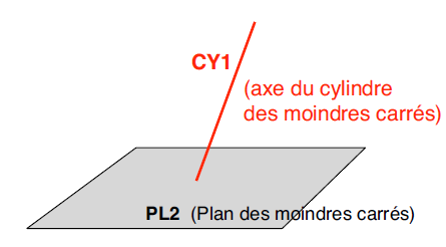
\includegraphics[width=0.4\linewidth]{img/Picture18}
\end{center}
}}

{\frame{
\frametitle{Contrôle d'une spécification géométrique 
\includegraphics[height=0.4cm]{img/Picture17}}

\begin{itemize}
\item L'axe réel du cylindre est déterminé par les 2 points extrêmes $PT8$ et $PT9$ délimitant l'axe du cylindre des moindres carrés,
 \item Etapes du processus
 \begin{itemize}
 \item construction du point $PT3$: intersection de la droite $CY1$ et du plan $PL2$,
 \item construction d'un axe orienté défini par: (une direction : le plan $PL2$, une origine : le point $PT3$, une orientation extérieure a la matière du plan $PL2$),
 \item construction de deux points $PT4$ et $PT5$ de coordonnées $-5$ et $-35$ (géométrie nominale),
 \item construction d'un plan $PL6$ passant par le point $PT4$ et parallèle au plan $PL2$,
 \item construction d'un plan $PL7$ passant par le point $PT5$ et parallèle au plan $PL2$,
 \item construction du point $PT8$ intersection de $PL6$ et de la droite $CY1$,
 \item construction du point $PT9$ intersection de $PL7$ et de la droite $CY1$
\end{itemize}
\end{itemize}

\begin{center}
 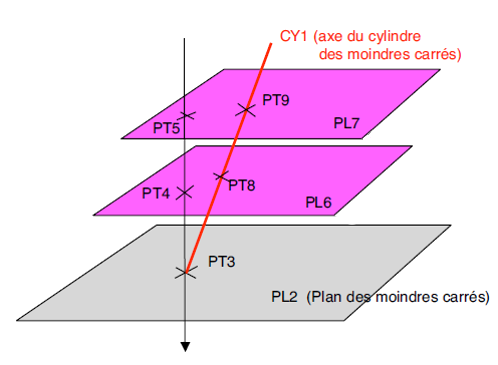
\includegraphics[width=0.4\linewidth]{img/Picture19}
\end{center}
}}

{\frame{
\frametitle{Contrôle d'une spécification géométrique 
\includegraphics[height=0.4cm]{img/Picture17}}

\begin{itemize}
 \item La direction du plan de référence spécifié est déterminée par le plan des moindres carrés,
 \item L'axe de la zone de tolérance est définie par une droite $DR10$,
 \begin{itemize}
  \item construction d'une droite $DR10$ passant par $PT8$ et perpendiculaire au plan $PL2$,  
 \end{itemize}
 \item La condition d'appartenance à la zone de tolérance Øt est définie par :
 \begin{itemize}
  \item le calcul de la distance d entre le point $PT9$ et la droite $DR10$,
  \item la condition $d \leq t$.
 \end{itemize}
\end{itemize}

\begin{center}
 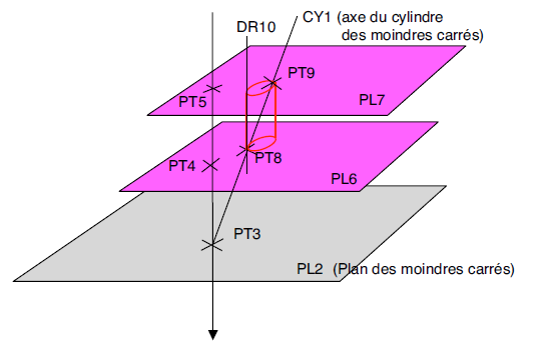
\includegraphics[width=0.4\linewidth]{img/Picture20}
\end{center}
}}

{\frame{
\frametitle{Technologies classiques de numérisation 3D}

\begin{itemize}
 \item Palpeur à déclanchement (contact) \\
 \begin{center}
 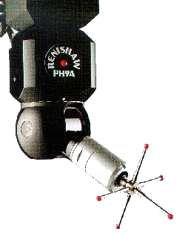
\includegraphics[height=2cm]{img/Picture21} 
 \end{center}
 \item Palpeur laser plan (sans contact) \\
 \begin{center}
 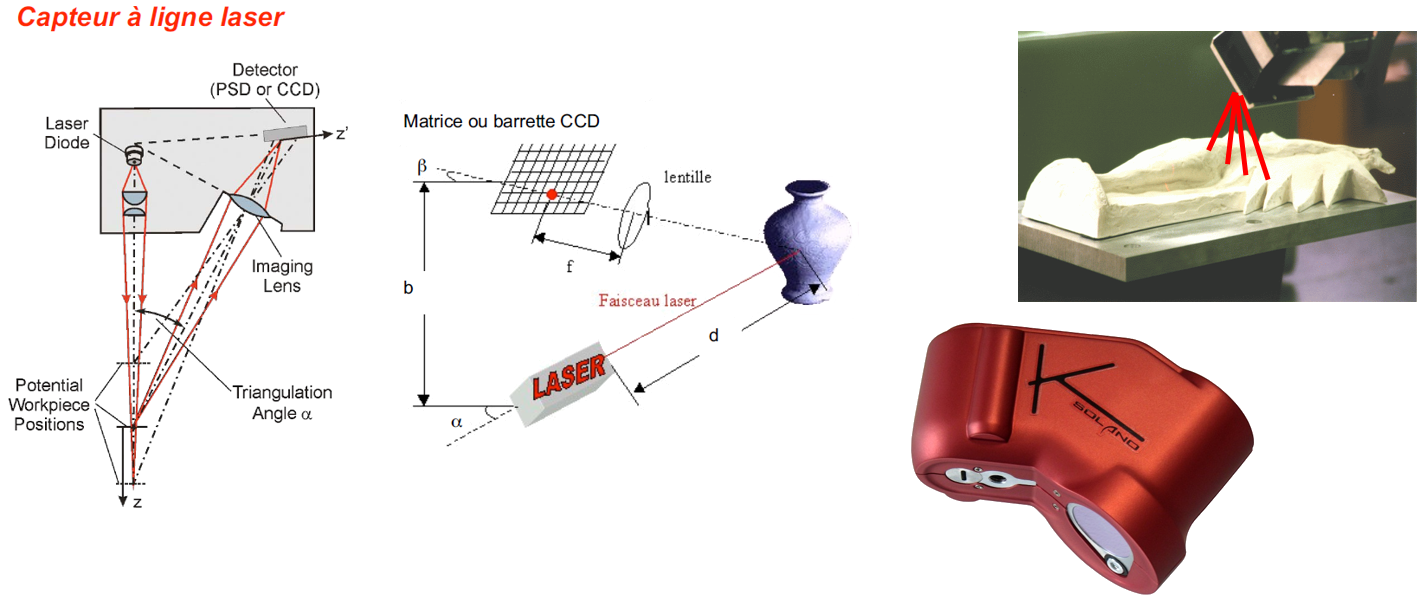
\includegraphics[height=3cm]{img/Picture22} 
 \end{center}
\end{itemize}
}}

{\frame{
\frametitle{Technologies et numérisation 3D grande échelle}

 
\includegraphics[width=0.8\linewidth]{img/Picture23}
}}

\section{Métrologie au marbre}

{\frame{
\frametitle{La métrologie au marbre: Méthode de mesure par comparaison}

\begin{minipage}[t]{0.45\linewidth}
\begin{itemize}
 \item Principe
  \begin{itemize}
  \item Contrôler une spécification dimensionnelle sur une pièce en la comparant à un empilement de cales étalon,
  \end{itemize}
 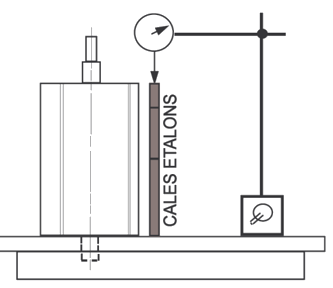
\includegraphics[width=0.7\linewidth]{img/Picture24}
 \item Etalonnage:
 \begin{itemize}
  \item Empiler les cales étalons pour atteindre la valeur nominale à mesurer,
  \item Amener le comparateur sur la pièce, il doit être à mi-course.
 \end{itemize}
\end{itemize}
\end{minipage}\hfill
\begin{minipage}[t]{0.45\linewidth}
\begin{itemize}
 \item Matériel utilisé:
 \begin{itemize}
  \item Un marbre de contrôle,
  \item Un jeu de cale étalon,
  \item Un comparateur+ support,
 \end{itemize}
 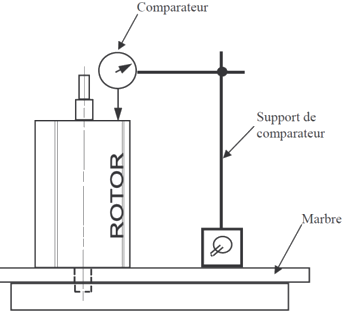
\includegraphics[width=0.7\linewidth]{img/Picture25}
 \item Procédure de mesure:
 \begin{itemize}
  \item Enlever les cales,
  \item Installer la pièce,
  \item Relever l'écart par rapport à l'étalonnage en bougeant la pièce.
 \end{itemize}
\end{itemize}
\end{minipage}
}}

{\frame{
\frametitle{Instruments de métrologie au marbre}

\begin{itemize}
 \item \textbf{Pied à coulisse:} Un pied à coulisse est un instrument de mesure de longueurs composée de deux parties coulissantes l'une sur l'autre : un règle fixe graduée, munie d'une tête comportant une face plate correspondant à la position de référence 0, et un curseur, muni d'une tête présentant une surface plate en opposition avec la référence.
\end{itemize}

\begin{center}
 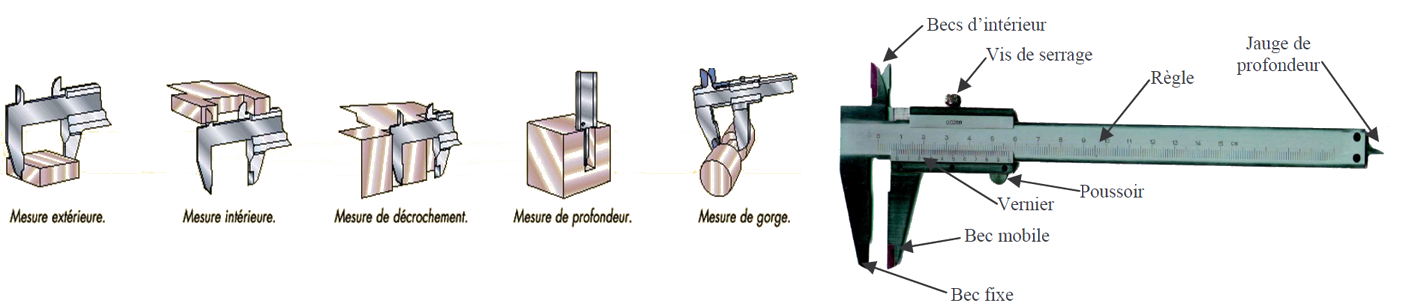
\includegraphics[width=0.8\linewidth]{img/Picture26} \\
 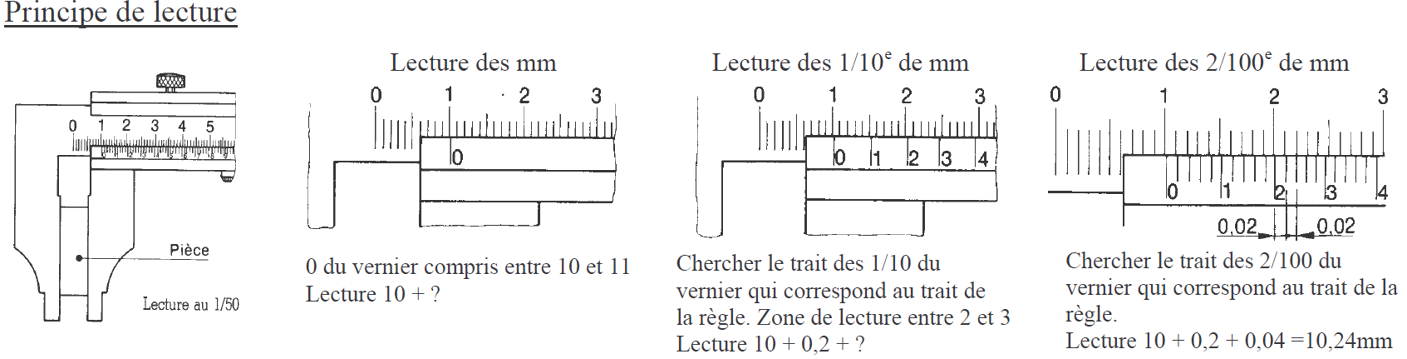
\includegraphics[width=0.8\linewidth]{img/Picture27}
\end{center}
}}

{\frame{
\frametitle{Instruments de métrologie au marbre}

\begin{itemize}
 \item \textbf{Micromètre:} Le micromètre, ou \og palmer \fg, est un appareil de mesure des longueurs. Il est très utilisé en mécanique pour mesurer des épaisseurs, des diamètres de portées cylindriques (micromètre d'extérieur) ou des diamètres de perçage ou d'alésage (micromètre d'intérieur).
\end{itemize}

\begin{center}
 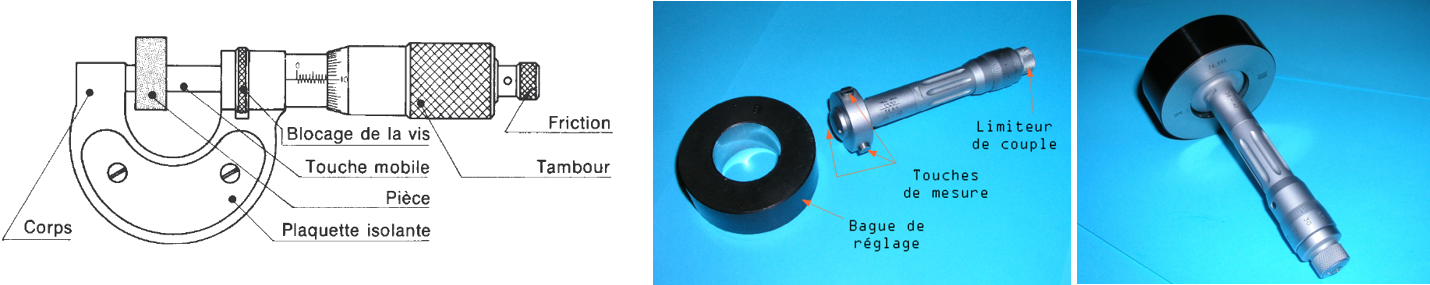
\includegraphics[width=0.8\linewidth]{img/Picture28} \\
 
\includegraphics[width=0.8\linewidth]{img/Picture29}
\end{center}
}}

{\frame{
\frametitle{Instruments de métrologie au marbre}

\begin{itemize}
 \item \textbf{Comparateur:} Le comparateur est un appareil de mesure de longueur. Il n'indique pas une mesure absolue mais une mesure relative par rapport à un point de référence, \\
  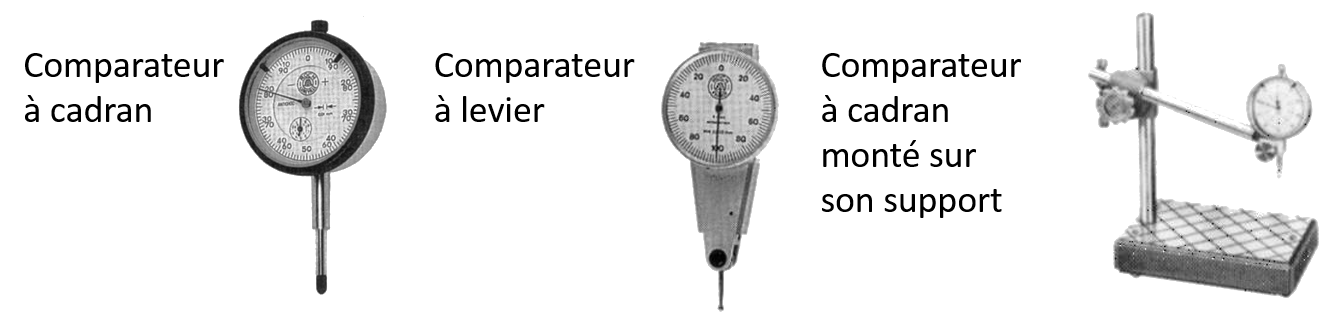
\includegraphics[width=0.8\linewidth]{img/Picture30}
 \item \textbf{Cales étalons:} Les cales étalons sont des parallélépipèdes généralement en acier dont la longueur entre deux des faces (appelées mesurandes) est parfaitement connue. Les cales étalons sont utilisées pour étalonner ou régler des appareils de mesure de longueur. \\
  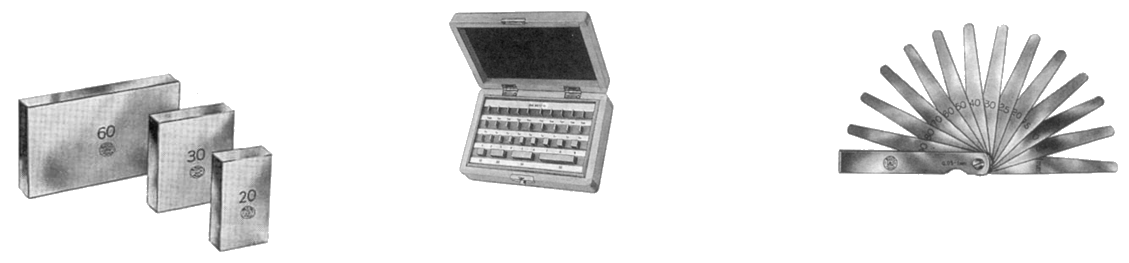
\includegraphics[width=0.8\linewidth]{img/Picture31}
\end{itemize}
}}

{\frame{
\frametitle{La métrologie}

\begin{savoir}
Vous devez être capables :
\begin{itemize}
 \item de mesurer les défauts d'une pièce,
 \item de construire un protocole de mesure.
\end{itemize}
\end{savoir}

\vfill

}}


\end{document}